\chapter{Benchmark}

\section{TrainBenchmark}

The base of my work was a benchmark named \textit{TrainBenchmark} developed by Benedek Izsó, István Ráth and Zoltán Szatmári. The goal of the TrainBenchmark is to compare EMF-IncQuery \cite{incquery} to other (preferably incremental) query tools.

The TrainBenchmark defines two scenarios:

\begin{description}
  \item[UserScenario] This scenario simulates a user sitting in front of her workstation and modifying the model in small steps.
  \item[XFormScenario] This scenario simulates a software running automated transformations on the model.
\end{description}

\subsection{Metamodel}

TrainBenchmark works on a railroad's model. The metamodel is shown on \autoref{fig:metamodel}.

\begin{figure}
\begin{center}
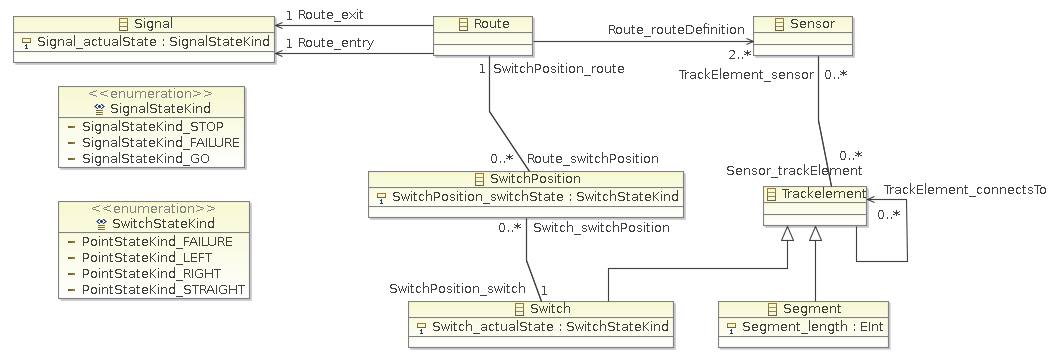
\includegraphics[width=14cm]{figures/TrainMetamodel}
\caption{The metamodel for the TrainBenchmark}
\label{fig:metamodel}
\end{center}
\end{figure}

The \texttt{generator} project of TrainBenchmark is capable of generating railroad instance models of different sizes. The project contains classes for generating models in different formats, including EMF, OWL, RDF and SQL.

\section{Queries}

The queries in TrainBenchmark look for violations of well-formedness constraints in the model. We only discuss the \textit{RouteSensor} query in detail.

\subsection{RouteSensor}

The \textit{RouteSensor} query looks for \textit{Sensors} that are connected to a \textit{Switch}, but the sensor and the switch are \textit{not} connected to the same \textit{Route}. The graphical representation of the RouteSensor query is shown on \autoref{fig:routesensor}.

\begin{figure}
\begin{center}
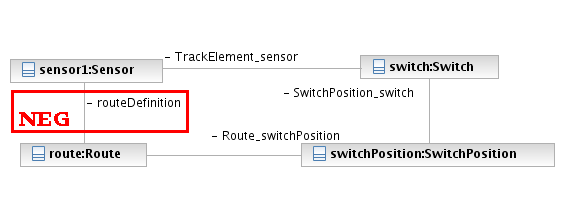
\includegraphics[]{figures/OD_RouteSensor}
\caption{Graphical representation of the RouteSensor query}
\label{fig:routesensor}
\end{center}
\end{figure}

The Cypher code for all TrainBenchmark queries is shown in detail in \autoref{cypherqueries}.

\section{Phases}

The TrainBenchmark consists of the following phases:

\begin{enumerate}
  \item $read$: loading the model,
  \item $check_0$: running the queries,
  \item $edit_i$: editing the model, 
  \item $check_i$: running the queries again.
\end{enumerate}

In a ,,real-world'' model editing sequence, the user tipically edits the model in small steps ($edit_i$ phases). The user's work is much more productive if she receives an instant feedback, hence we would like to run re-evaluate well-formedness queries quickly (preferably in sub-second time). This creates the need for an incremental pattern matcher tools.

\section{Neo4j}

NoSQL database management system come in many flavor, including \textit{graph databases} \cite{NoSQL}. Neo4j is the most popular and most funded graph database on the market today. Neo4j is developed by a Swedish company Neo Technology since 2002 \cite{neo4j}. It's available as an open source project since 2007.

\begin{figure}
\begin{center}

\includegraphics[]{figures/neo4j-logo}
\caption{The logo of Neo4j}
\label{fig:neo4j-logo}
\end{center}
\end{figure}

Neo4j graphs can be visualised in Neoclipse, an Eclipse RCP application \cite{Neoclipse}.

\begin{figure}
\begin{center}
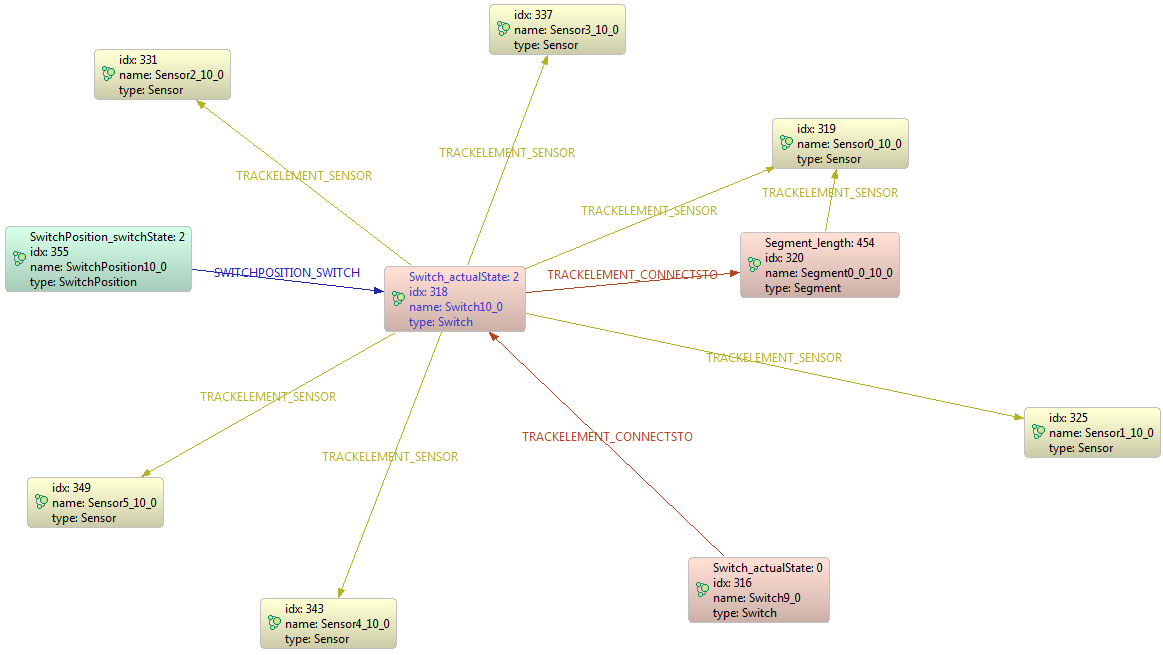
\includegraphics[width=14cm]{figures/neoclipse-graph}
\caption{A subgraph of a TrainBenchmark instance visualised in Neoclipse}
\label{fig:neoclipse}
\end{center}
\end{figure}

The lack of a common formal data model is both an advantage and a shortcoming of NoSQL databases. The Tinkerpop framework \cite{Tinkerpop} aims to provide a common data model and interface for graph databases.

\section{Generation of models}

I created a property graph generator project based on the previous TrainBenchmark generators. The generator creates a graph in an embedded Neo4j database and uses the Blueprints library's \texttt{GraphMLWriter} class to save to a GraphML file \cite{Blueprints}.

\subsection{RouteSensor}

The Cypher implementation of the RouteSensor query is shown on \autoref{lst:cypher-routesensor}

\begin{lstlisting}[caption=Cyper query for the RouteSensor test case, label=lst:cypher-routesensor, breaklines=true]
START sensor=node:node_auto_index(type="Sensor")
MATCH sensor-[:TRACKELEMENT_SENSOR]-switch-[:SWITCHPOSITION_SWITCH]-switchPosition-[:ROUTE_SWITCHPOSITION]-route-[r?:ROUTE_ROUTEDEFINITION]-sensor
WHERE r IS NULL
RETURN sensor
\end{lstlisting}
